\chapter*{Vlastní implementace}

\par Součástí úlohy bylo kromě samotných algoritmů analyzujících polohu bodu v prostoru také vytvoření přívětivého uživatelského prostředí ve frameworku QT, ve kterém je demonstrována funkčnost obou výše zmíněných algoritmů
na zvolené polygonové mapě. 

\section*{Vstupní data}
\par Jako vstupní data byly zvoleny geografická data s kódem \verb|EPSG:5514| (Křovákovo zobrazení). Aplikace umožňuje otevřít, zpracovat a vykreslit prostorové souřadnice pro soubory ve formátu \verb|.JSON| a \verb|.GEOJSON|. K aplikaci jsou přiloženy testovací data v obou formátech v adresáři \emph{/input\textunderscore files/}.
\par Výsledkem analýzy je grafické vykreslení příslušnosti bodu k polygonu, případně k více polygonům v situaci, kdy je bod umístěn na rozhraní dvou nebo více polygonů.

\bigbreak

\section*{Aplikace}
\par Grafické rozhraní aplikace (obrázek 3) bylo vytvořeno v prostředí \verb|Qt Creator 9.0.1| a dále upravováno v prostředí programovacího jazyka \verb|Python 3.11|. Uživateli je umožněno otevřít soubor ve vlastním adresáři a v těle aplikace kliknutím levého tlačítka myši umístit vlastní bod $q$ pro analýzu jeho polohy vůči vstupním datům. 

\begin{figure}[h]
    \centering
        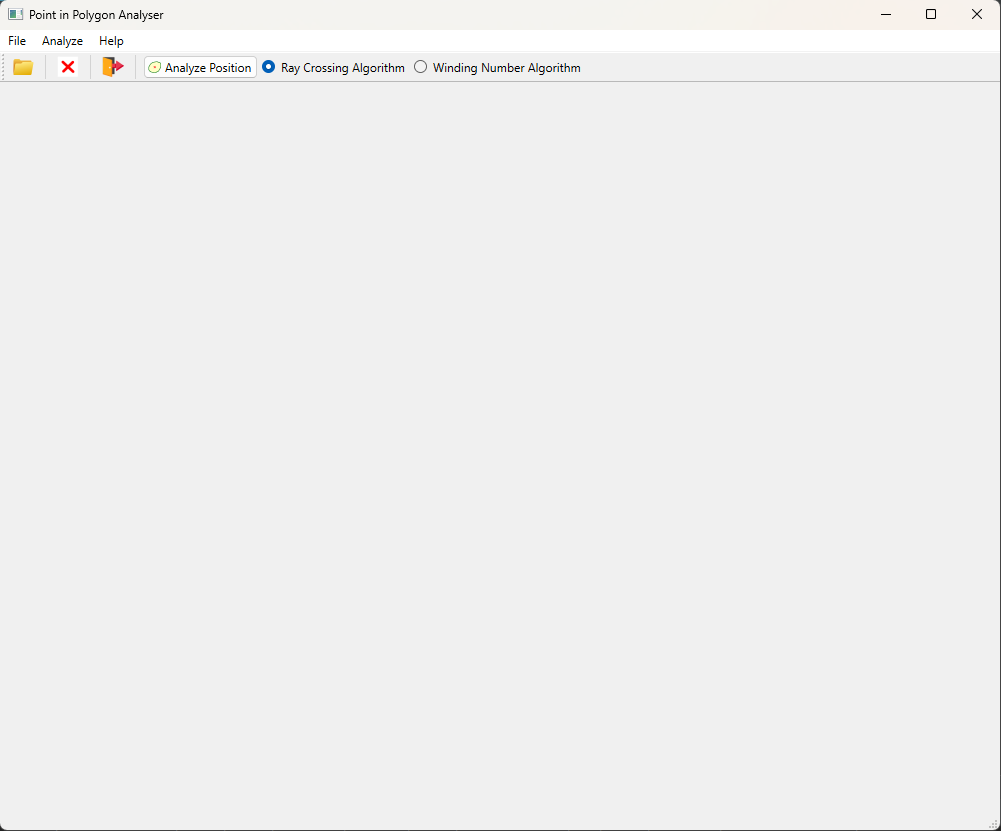
\includegraphics[width=10cm]{aplikace} 
        \caption{Grafické rozhraní aplikace}
\end{figure}

\par Součástí rozhraní je možnost volby matoedy analýzy mezi algoritmy \emph{Ray Crossing} a \emph{Winding Number} (obrázek 4). Po zvolení algoritmu a kliknutí na \verb|Analyze Position| (případně využití klávesové zkratky \verb|Ctrl+A|) se zvýrazní polygon, ve kterém se bod $q$ nachází. V případě, že se bod $q$ nachází na hraně dvou polygonů, resp. na rozhraní více polygonů, zvýrazní se všechny incidující polygony.

\begin{figure}[h]
    \centering
        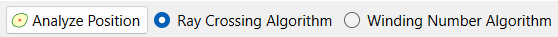
\includegraphics[width=10cm]{toolbar} 
        \caption{Panel nástrojů pro volbu algoritmů}
\end{figure}

\par Uživatel má také možnost vstupní polygonovou vrstvu smazat a nahrát novou vrstvu. V případě otevření nového souboru se předešlá vrstva smaže a nahraje se vrstva nová.
\par Vstupní vrstva se nahraje tak, aby vyplnila co nejvíc prostoru v okně aplikace (obrázek 5). S měnící se velikosti okna se ale již nahraná vrstva nemění, je tedy nutno znovu otevřít soubor tak, aby se data vhodně přeškálovala vzhledem k nové velikosti okna. 

\begin{figure}[h]
    \centering
        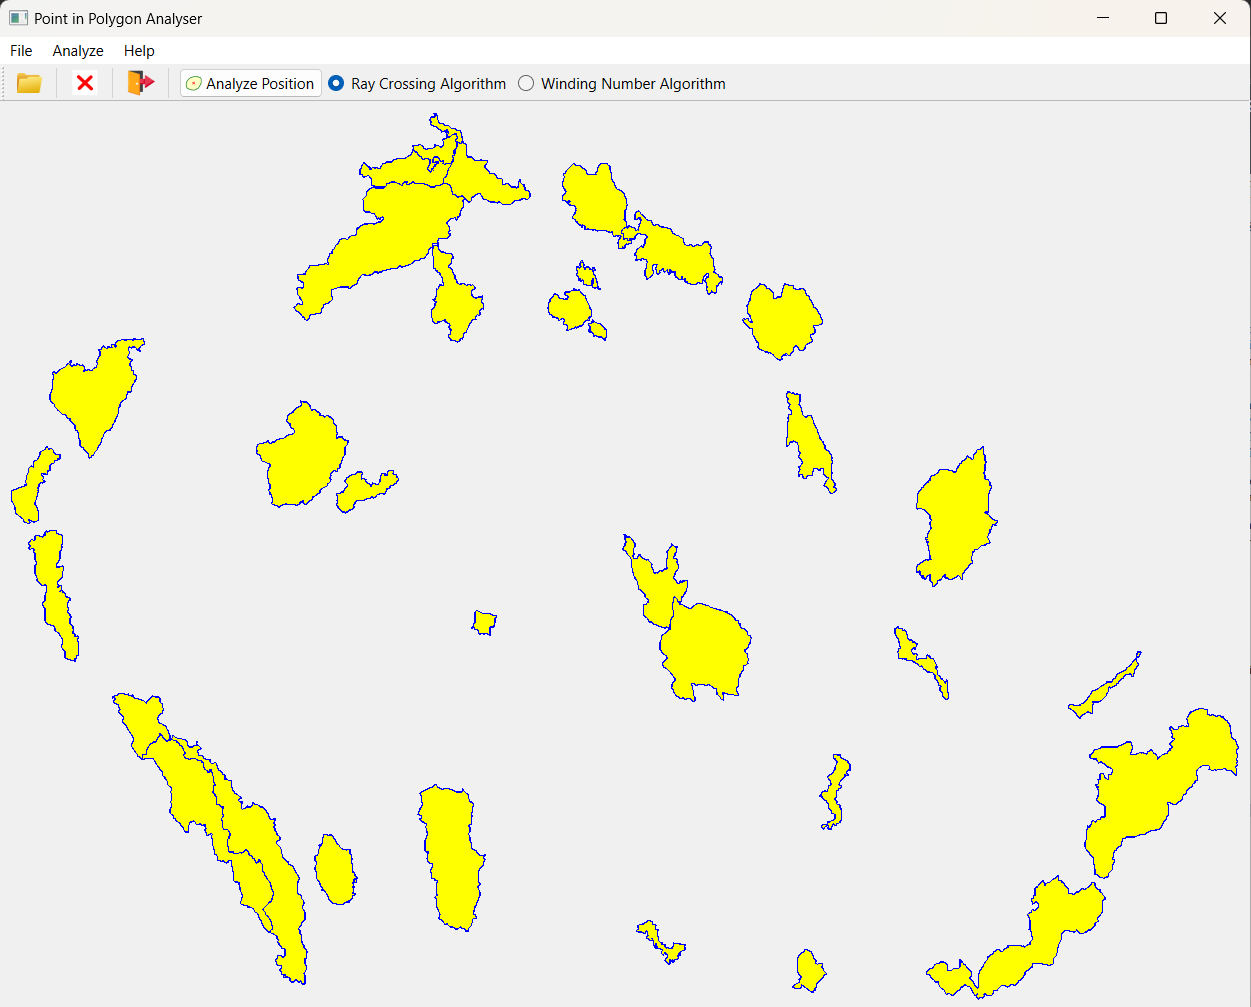
\includegraphics[width=12cm]{showcase} 
        \caption{Ukázka nahrané polygonové vrstvy}
\end{figure}
\par Polygon, ve kterém se zvolený bod může nacházet, se zabarví na modrou barvu. Pokud se zvolený bod nachází na hraně dvou polygonů nebo na vrcholu více polygonů, na tuto skutočnost upozorní vyskakovací okno (obrázek 6) a všechny tyto polygony se zabarví na modrou barvu.

\begin{figure}[h]
    \centering
        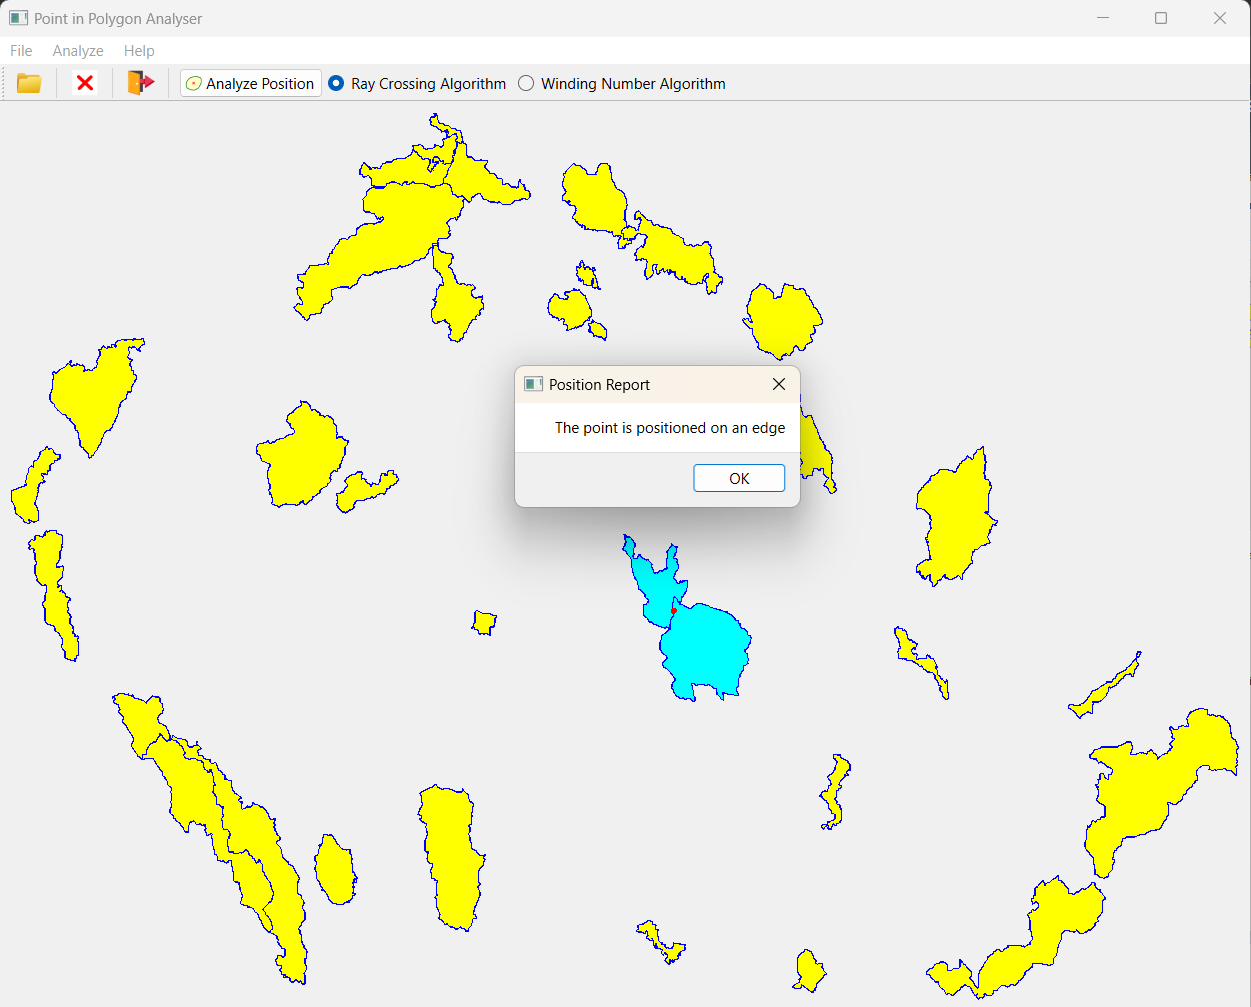
\includegraphics[width=10cm]{highlight} 
        \caption{Vyskakovací okno při detekci hrany}
\end{figure}

\bigbreak

\newpage
\section*{Třídy a metody}
\par Funkční chod aplikace si vyžaduje tři povinné soubory, v kterých jsou implementovány potřebné třídy a metody: \verb|mainform.py|, \verb|algorithms.py| a \verb|draw.py|.

\bigbreak

\par {\large\textbf{Třída MainForm} }
\par Třída MainForm ze souboru \verb|mainform.py| zabezpečuje inicializaci okna aplikace, vrchní lišty, panelu nástrojů, ikon a tlačítek. Zároveň přepojuje jednotlivé interaktivní položky okna s metodami, které vykonají specifické akce. Týkají se především otevření souboru, přepínání algoritmů, provedení analýzy polohy bodu vůči polygonu apod. Část této třídy byla vygenerována v prostředí \verb|Qt Creator 9.0.1| (metody \verb|setupUi()| a \verb|translateUi()|). Níže jsou vyjmenovány nově implementované metody:

\begin{itemize}
    \item \verb|switchToRayCrossing()|
        \subitem{Nastaví algoritmus pro analýzu polohy bodu na \emph{Ray Crossing}.}
    \item \verb|switchToWindingNumber()|
        \subitem{Nastaví algoritmus pro analýzu polohy bodu na \emph{Winding Number}.}
    \item \verb|analyzePosition()|
        \subitem{Provede analýzu polohy bodu $q$ vůči polygonové mapě. Bod a polygonovou mapu (uloženou v seznamu) zavolá z třídy \verb|Draw|. V iteraci přiřadí každému polygonu hodnotu, podle které se polygon zabarví a určí se tak jeho vztah k bodu $q$. Může zavolat metodu pro vyskakovací okno \verb|onEdgePopup()| .}
    \item \verb|processFile()|
        \subitem{Zabezpečuje otevření souboru. Samotný soubor načte do proměnné pomocí metody \verb|openFile()| a následně zavolá metodu \verb|clearEvent()| pro vyprázdnění okna. Pokud je vstupní \verb|JSON| nebo \verb|GeoJSON| nečitelný (např. nestandardní hierarchie položek v slovnících), uživatele na to upozorní vyskakovacím oknem.}
    \item \verb|openFile()|
        \subitem{Otevře \verb|JSON| nebo \verb|GeoJSON| soubor a načte ho do proměnné.}
    \item \verb|exitClick()|
        \subitem{Ukončí aplikaci.}
    \item \verb|clearClick()|
        \subitem{Zavolá metodu \verb|clearEvent()| z třídy \verb|Draw|, která vyprázdní okno.}
    \item \verb|aboutClick()|
        \subitem{Otevře repozitář s aplikací v portálu \verb|GitHub|.}
    \item \verb|onEdgePopup()|
        \subitem{Vytvoří vyskakovací okno v případě, že se zvolený bod nachází na hraně nebo na vrcholu polygonu.}
\end{itemize}

\bigbreak

\par {\large\textbf{Třída Algorithms} }
\par V této třídě jsou obsaženy metody, které byly detailně popsány v předchozí kapitole věnované teorii algoritmů Winding Number a Ray Crossing. Obsahuje metody:

\begin{itemize}
    \item \verb|rayCrossingAlgorithm(q, pol)|,
        \subitem{pro předané parametry \verb|q| (bod) a \verb|pol| (polygon) analyzuje polohu bodu \verb|q| vůči polygonu \verb|pol| pomocí algoritmu Ray Crossing}
    \item \verb|windingNumberAlgorithm(q, pol)|
        \subitem{pro předané parametry \verb|q| (bod) a \verb|pol| (polygon) analyzuje polohu bodu \verb|q| vůči polygonu \verb|pol| pomocí algoritmu Winding Number}
\end{itemize}

\par Třída obsahuje jednu proměnnou \verb|default_alg|, která nastavuje metodu rayCrossingAlgorithm jako primární metodu pro analýzu bodu a polygonu.

\bigbreak

\par {\large\textbf{Třída Draw} }
\par Třída Draw ze souboru \verb|Draw.py| slouží pro inicializaci proměnných nesoucí prostorovou informaci, načítání a vykreslování geoprostorové informace. Při spuštění aplikace se inicializují proměnné pro bod, polygonový list a polygonový status:

\begin{itemize}
  \item \verb|self.__q|,
  \item \verb|self.__polyg_list|,
  \item \verb|self.polyg_status|,
\end{itemize}

\par Třída Draw obsahuje následující metody:
\begin{itemize}
    \item \verb|mousePressEvent(e:QMouseEvent)|
        \subitem{Zodpovídá za změnu pozice bodu.}
    \item \verb|paintEvent(e:QPaintEvent)|
        \subitem{Vykresluje objekty (bod a polygony) na plátno (Canvas).}
    \item \verb|getPoint()|
        \subitem{Vrací souřadnice bodu.}
    \item \verb|getPolygonList()|
        \subitem{Vrací seznam vstupních polygonů.}
    \item \verb|clearEvent()|
        \subitem{Maže vyreslené objekty (bod a polygony) na plátně (Canvas).}
    \item \verb|findBoundingPoints(p:QPointF, xmin, ymin, xmax, ymax)|
        \subitem{Nalezne minimální a maximální souřadnice pro ohraničení polygonu (tzv. bounding box).}
    \item \verb|resizePolygons(xmin, ymin, xmax, ymax)|
        \subitem{Roztáhne vstupní data na plátno podle velikosti okna aplikace.}
    \item \verb|loadData(data)|
        \subitem{Prochází slovník ze vstupního souboru \verb|.JSON/.GEOJSON| a načítá geoprostorovou informaci.}
\end{itemize}
